% 9pt, 10pt, 11pt, 12pt, 14pt, 17pt, 21pt, 25pt, 30pt, 36pt, 43pt
\documentclass[9pt,a4paper,]{ltjsarticle}
% ページの余白設定

% ページ全体の行間設定
% ref: http://d.hatena.ne.jp/pureodio/20100929/1285736949

  
  \makeatletter
  \@ifpackageloaded{subfig}{}{\usepackage{subfig}}
  \@ifpackageloaded{caption}{}{\usepackage{caption}}
  \captionsetup[subfloat]{margin=0.5em}
  \AtBeginDocument{%
  \renewcommand*\figurename{図}
  \renewcommand*\tablename{表}
  }
  \AtBeginDocument{%
  \renewcommand*\listfigurename{List of Figures}
  \renewcommand*\listtablename{List of Tables}
  }
  \@ifpackageloaded{float}{}{\usepackage{float}}
  \floatstyle{ruled}
  \@ifundefined{c@chapter}{\newfloat{codelisting}{h}{lop}}{\newfloat{codelisting}{h}{lop}[chapter]}
  \floatname{codelisting}{コード}
  \newcommand*\listoflistings{\listof{codelisting}{List of Listings}}
  \makeatother

% 数式ライブラリ
\usepackage{amssymb,amsmath}

% SI単位系
% usable: \si{ \any }
% e.g.) \si{ \decibel }
\usepackage{siunitx}

% 表組みの横幅指定やセル内の書式指定など
\usepackage{tabularx}

% 英文の印刷物では, 最初のパラグラフの字下げはしないらしいので対応
\usepackage{indentfirst}

% 不明
\usepackage{ragged2e}

% 表のセルを縦に結合
\usepackage{multirow}

% 不明
\usepackage{gensymb}

% テキストシンボル
% ref: http://www.yamamo10.jp/yamamoto/comp/latex/make_doc/symbol/index.php#TEXTCOMP
\usepackage{textcomp}

% フォント設定
\usepackage{lmodern}

\usepackage{ifxetex,ifluatex}

\usepackage{fixltx2e} % provides \textsubscript
\ifnum 0\ifxetex 1\fi\ifluatex 1\fi=0 % if pdftex
\usepackage[T1]{fontenc}
\usepackage[utf8]{inputenc}
\else % if luatex or xelatex
\ifxetex
\usepackage{mathspec}
\else
\usepackage{fontspec}
\fi
\defaultfontfeatures{Mapping=tex-text,Scale=MatchLowercase}
\newcommand{\euro}{€}





\fi
% use upquote if available, for straight quotes in verbatim environments
\IfFileExists{upquote.sty}{\usepackage{upquote}}{}
% use microtype if available
\IfFileExists{microtype.sty}{%
\usepackage{microtype}
\UseMicrotypeSet[protrusion]{basicmath} % disable protrusion for tt fonts
}{}

\makeatletter
\newcommand*{\rom}[1]{\expandafter\@slowromancap\romannumeral #1@}
\makeatother

\newcommand{\fracTable}[2]{\vtop{\hbox{\strut #1}\hbox{\strut #2}}}

\newcommand*{\unit}[1]{\mathrm{\ [#1]}}

\makeatletter
\def\fps@figure{h}
\@ifpackageloaded{hyperref}{}{%
\ifxetex
  \usepackage[setpagesize=false, % page size defined by xetex
              unicode=false, % unicode breaks when used with xetex
              xetex]{hyperref}
\else
  \usepackage[unicode=true]{hyperref}
\fi
}
\@ifpackageloaded{color}{
    \PassOptionsToPackage{usenames,dvipsnames}{color}
}{%
    \usepackage[usenames,dvipsnames]{color}
}

\makeatother
\hypersetup{breaklinks=true,
            bookmarks=true,
            pdfauthor={},
            pdftitle={},
            colorlinks=true,
            citecolor=blue,
            urlcolor=blue,
            linkcolor=magenta,
            pdfborder={0 0 0}
            }
\urlstyle{same}  % don't use monospace font for urls



\usepackage{color}
\usepackage{fancyvrb}
\newcommand{\VerbBar}{|}
\newcommand{\VERB}{\Verb[commandchars=\\\{\}]}
\DefineVerbatimEnvironment{Highlighting}{Verbatim}{commandchars=\\\{\}}
% Add ',fontsize=\small' for more characters per line
\newenvironment{Shaded}{}{}
\newcommand{\AlertTok}[1]{\textcolor[rgb]{1.00,0.00,0.00}{\textbf{#1}}}
\newcommand{\AnnotationTok}[1]{\textcolor[rgb]{0.38,0.63,0.69}{\textbf{\textit{#1}}}}
\newcommand{\AttributeTok}[1]{\textcolor[rgb]{0.49,0.56,0.16}{#1}}
\newcommand{\BaseNTok}[1]{\textcolor[rgb]{0.25,0.63,0.44}{#1}}
\newcommand{\BuiltInTok}[1]{#1}
\newcommand{\CharTok}[1]{\textcolor[rgb]{0.25,0.44,0.63}{#1}}
\newcommand{\CommentTok}[1]{\textcolor[rgb]{0.38,0.63,0.69}{\textit{#1}}}
\newcommand{\CommentVarTok}[1]{\textcolor[rgb]{0.38,0.63,0.69}{\textbf{\textit{#1}}}}
\newcommand{\ConstantTok}[1]{\textcolor[rgb]{0.53,0.00,0.00}{#1}}
\newcommand{\ControlFlowTok}[1]{\textcolor[rgb]{0.00,0.44,0.13}{\textbf{#1}}}
\newcommand{\DataTypeTok}[1]{\textcolor[rgb]{0.56,0.13,0.00}{#1}}
\newcommand{\DecValTok}[1]{\textcolor[rgb]{0.25,0.63,0.44}{#1}}
\newcommand{\DocumentationTok}[1]{\textcolor[rgb]{0.73,0.13,0.13}{\textit{#1}}}
\newcommand{\ErrorTok}[1]{\textcolor[rgb]{1.00,0.00,0.00}{\textbf{#1}}}
\newcommand{\ExtensionTok}[1]{#1}
\newcommand{\FloatTok}[1]{\textcolor[rgb]{0.25,0.63,0.44}{#1}}
\newcommand{\FunctionTok}[1]{\textcolor[rgb]{0.02,0.16,0.49}{#1}}
\newcommand{\ImportTok}[1]{#1}
\newcommand{\InformationTok}[1]{\textcolor[rgb]{0.38,0.63,0.69}{\textbf{\textit{#1}}}}
\newcommand{\KeywordTok}[1]{\textcolor[rgb]{0.00,0.44,0.13}{\textbf{#1}}}
\newcommand{\NormalTok}[1]{#1}
\newcommand{\OperatorTok}[1]{\textcolor[rgb]{0.40,0.40,0.40}{#1}}
\newcommand{\OtherTok}[1]{\textcolor[rgb]{0.00,0.44,0.13}{#1}}
\newcommand{\PreprocessorTok}[1]{\textcolor[rgb]{0.74,0.48,0.00}{#1}}
\newcommand{\RegionMarkerTok}[1]{#1}
\newcommand{\SpecialCharTok}[1]{\textcolor[rgb]{0.25,0.44,0.63}{#1}}
\newcommand{\SpecialStringTok}[1]{\textcolor[rgb]{0.73,0.40,0.53}{#1}}
\newcommand{\StringTok}[1]{\textcolor[rgb]{0.25,0.44,0.63}{#1}}
\newcommand{\VariableTok}[1]{\textcolor[rgb]{0.10,0.09,0.49}{#1}}
\newcommand{\VerbatimStringTok}[1]{\textcolor[rgb]{0.25,0.44,0.63}{#1}}
\newcommand{\WarningTok}[1]{\textcolor[rgb]{0.38,0.63,0.69}{\textbf{\textit{#1}}}}
\usepackage{graphicx,grffile}
\makeatletter
\def\maxwidth{\ifdim\Gin@nat@width>\linewidth\linewidth\else\Gin@nat@width\fi}
\def\maxheight{\ifdim\Gin@nat@height>\textheight\textheight\else\Gin@nat@height\fi}
\makeatother
% Scale images if necessary, so that they will not overflow the page
% margins by default, and it is still possible to overwrite the defaults
% using explicit options in \includegraphics[width, height, ...]{}
\setkeys{Gin}{width=\maxwidth,height=\maxheight,keepaspectratio}
\setlength{\parindent}{0pt}
\setlength{\parskip}{6pt plus 2pt minus 1pt}
\setlength{\emergencystretch}{3em}  % prevent overfull lines
\providecommand{\tightlist}{%
  \setlength{\itemsep}{0pt}\setlength{\parskip}{0pt}}
\setcounter{secnumdepth}{5}

\begin{document}
% % 
% ------------------------------------

% LaTeXのタイプセットで生成されるファイル群の処理
% .toc: \tableofcontents コマンドが記載されたときにタイプセットされる目次情報を書き出したファイル。

% .lot: \listoftable コマンドが記載されたときにタイプセットされる表情報を書き出したファイル。

% .lof: \listoftable コマンドが記載されたときにタイプセットされる図情報を書き出したファイル。

% Custom template starts from here
\newenvironment{boldtabular}{ \arrayrulewidth = 2pt }{}
\newenvironment{narrowtabular}{ \renewcommand{\arraystretch}{0.8} }{}
\newenvironment{titletabular}{ \renewcommand{\arraystretch}{1.1} }{}
\newenvironment{datetabular}{ \renewcommand{\arraystretch}{1.1} }{}
\newenvironment{templaturetabular}{ \renewcommand{\arraystretch}{1.18} }{}
\newenvironment{report-title}{
\centering
  \fontsize{20pt}{20pt}\selectfont
}{}
\fontsize{14pt}{28pt}\selectfont

\begin{center}
  \begin{report-title}
    \textbf{Report on the Experiment}
  \end{report-title}

  \vspace{10mm}

  \textbf{No.} \textbf{9}\\

  \vspace{10mm}

  \textbf{Subject} \textbf{dsPICマイコンプログラミング1}\\

  \vspace{10mm}

  \textbf{Date} \textbf{2021. 06. 23}\\

  \vspace{10mm}

  \textbf{Weather} \textbf{    腫れ    }
  \textbf{Temp} \textbf{    24.5 \celsius    }
  \textbf{Wet} \textbf{    62 \%    }
\end{center}

\vspace{10mm}

\begin{table}[!h]
  \begin{flushright}
    \begin{tabular}{rl}
      \textbf{Class}   & \textbf{ E5 } \\
      \textbf{Group}   & \textbf{ 4 } \\
      \textbf{Chief}   & \textbf{  } \\
      \textbf{Partner} & \textbf{  } \\
                       & \textbf{  } \\
                       & \textbf{  } \\
                       & \textbf{  }
    \end{tabular}
  \end{flushright}
\end{table}

\vspace{15mm}

\begin{table}[!h]
  \begin{flushright}
    \begin{tabular}{rl}
      \textbf{No}   & \textbf{ 14 } \\
      \textbf{Name} & \textbf{ 小畠 一泰 }
    \end{tabular}
  \end{flushright}
\end{table}


  % \makebox[15ex]{Censored text}\hspace{-15ex}
  % \makebox[\textwidth]{c e n t r a l} \par
  % \makebox[15ex]{\hrulefill}{Censored text}\hspace{-15ex}\raisebox{10pt}[20pt][30pt]

  % \textbf{Partner} \makebox[3in]{\textbf{        }}{\hrulefill}[c]
  % \begin{flushright}
  %   \textbf{Partner} \hspace{1cm} \underline{\textbf{        }}\\
  %   \underline{\textbf{        }}\\
  %   \underline{\textbf{        }}\\
  %   \underline{\textbf{        }}\\
  % \end{flushright}

\vspace{10mm}

\begin{center}
  \textbf{Kure National College of Technology}
\end{center}

\thispagestyle{empty}
\newpage
\setcounter{page}{1}

\normalsize

% end of custom template
\hypertarget{ux76eeux7684}{%
\section{目的}\label{ux76eeux7684}}

dsPIC を用いて, A/D 変換, タイマ機能と割り込み, PWM 出力の演習を行う.

\hypertarget{ux5b9fux9a13ux6a5fux5668}{%
\section{実験機器}\label{ux5b9fux9a13ux6a5fux5668}}

\begin{itemize}
\tightlist
\item
  マイコンボード
\item
  PC
\end{itemize}

\hypertarget{ux8ab2ux984c}{%
\section{課題}\label{ux8ab2ux984c}}

\hypertarget{ux8ab2ux984c-1}{%
\subsection{課題 1}\label{ux8ab2ux984c-1}}

\begin{codelisting}

\caption{課題 1 コード}

\hypertarget{lst:awesome-code}{%
\label{lst:awesome-code}}%
\begin{Shaded}
\begin{Highlighting}[numbers=left,,]
\PreprocessorTok{#include }\ImportTok{<p30F3013.h>}
\PreprocessorTok{#include }\ImportTok{"c:\textbackslash{}work\textbackslash{}lcd.h"}
\DataTypeTok{void}\NormalTok{ init_ADC() \{}
\NormalTok{  TRISBbits.TRISB1 = }\DecValTok{1}\NormalTok{;  }\CommentTok{// RB1 as input}
\NormalTok{  ADPCFG = }\BaseNTok{0xFFFD}\NormalTok{;}
\NormalTok{  ADCHS = }\BaseNTok{0x0001}\NormalTok{;}
\NormalTok{  ADCON1 = }\BaseNTok{0x0000}\NormalTok{;}
\NormalTok{  ADCSSL = }\DecValTok{0}\NormalTok{;}
\NormalTok{  ADCON2 = }\BaseNTok{0x0000}\NormalTok{;}
\NormalTok{  ADCON3 = }\BaseNTok{0x0013}\NormalTok{;}
\NormalTok{  ADCON1bits.ADON = }\DecValTok{1}\NormalTok{;  }\CommentTok{// ADC on}
\NormalTok{\}}
\DataTypeTok{unsigned} \DataTypeTok{int}\NormalTok{ get_ADC() \{}
\NormalTok{  ADCON1bits.SAMP = }\DecValTok{1}\NormalTok{;  }\CommentTok{// sampling start}
\NormalTok{  delayms(}\DecValTok{100}\NormalTok{);}
\NormalTok{  ADCON1bits.SAMP = }\DecValTok{0}\NormalTok{;  }\CommentTok{// converting start}
  \ControlFlowTok{while}\NormalTok{ (!ADCON1bits.DONE);}
  \ControlFlowTok{return}\NormalTok{ ADCBUF0;  }\CommentTok{// ADC value}
\NormalTok{\}}
\DataTypeTok{int}\NormalTok{ main() \{}
\NormalTok{  init_LCD();}
\NormalTok{  init_ADC();}
  \ControlFlowTok{while}\NormalTok{ (}\DecValTok{1}\NormalTok{) \{ clr_LCD();}
\NormalTok{    put_num(get_ADC());}
\NormalTok{    delayms(}\DecValTok{500}\NormalTok{);}
\NormalTok{  \}}
\NormalTok{\}}
\end{Highlighting}
\end{Shaded}

\end{codelisting}

\clearpage

\hypertarget{ux8ab2ux984c-2}{%
\subsection{課題 2}\label{ux8ab2ux984c-2}}

\begin{codelisting}

\caption{課題 2 コード(その1)}

\hypertarget{lst:awesome-code}{%
\label{lst:awesome-code}}%
\begin{Shaded}
\begin{Highlighting}[numbers=left,,]
\PreprocessorTok{#include }\ImportTok{<p30F3013.h>}
\PreprocessorTok{#include }\ImportTok{"c:\textbackslash{}work\textbackslash{}lcd.h"}

\DataTypeTok{int}\NormalTok{ Resultdata, Msec = }\DecValTok{0}\NormalTok{, flag = }\DecValTok{0}\NormalTok{;}

\DataTypeTok{void}\NormalTok{ init_adc() \{}
\NormalTok{  TRISBbits.TRISB1 = }\DecValTok{1}\NormalTok{;  }\CommentTok{// RB1 as input}
\NormalTok{  ADPCFG = }\BaseNTok{0xFFFD}\NormalTok{;}
\NormalTok{  ADCHS = }\BaseNTok{0x0001}\NormalTok{;}
\NormalTok{  ADCON1 = }\BaseNTok{0x0044}\NormalTok{;}
\NormalTok{  ADCSSL = }\DecValTok{0}\NormalTok{;}
\NormalTok{  ADCON2 = }\BaseNTok{0x0000}\NormalTok{;}
\NormalTok{  ADCON3 = }\BaseNTok{0x0113}\NormalTok{;}
\NormalTok{  ADCON1bits.ADON = }\DecValTok{1}\NormalTok{;  }\CommentTok{// ADC on}
\NormalTok{\}}

\DataTypeTok{void}\NormalTok{ _ISR _AltT3Interrupt(}\DataTypeTok{void}\NormalTok{) \{}
\NormalTok{  ++Msec;}
  \ControlFlowTok{if}\NormalTok{ (Msec >= }\DecValTok{1000}\NormalTok{) \{}
\NormalTok{    Msec = }\DecValTok{0}\NormalTok{;}
\NormalTok{    flag = }\DecValTok{1}\NormalTok{;}
\NormalTok{  \}}
  \ControlFlowTok{while}\NormalTok{ (!IFS0bits.ADIF);}
\NormalTok{  Resultdata = ADCBUF0;}
\NormalTok{  IFS0bits.ADIF = }\DecValTok{0}\NormalTok{;}
\NormalTok{  IFS0bits.T3IF = }\DecValTok{0}\NormalTok{;  }\CommentTok{// タイマ3割り込みフラグクリア}
\NormalTok{\}}

\DataTypeTok{void}\NormalTok{ init_timer() \{}
\NormalTok{  INTCON1bits.NSTDIS = }\DecValTok{0}\NormalTok{;}
\NormalTok{  INTCON2bits.ALTIVT = }\DecValTok{1}\NormalTok{;  }\CommentTok{// 代替ベクタを使用}
\NormalTok{  TMR3 = }\BaseNTok{0x0000}\NormalTok{;           }\CommentTok{// clear counter register}
\NormalTok{  PR3 = }\DecValTok{29480}\NormalTok{ - }\DecValTok{1}\NormalTok{;         }\CommentTok{// set period register (1kHz)}
\NormalTok{  IFS0 = }\BaseNTok{0x0000}\NormalTok{;           }\CommentTok{// clear all interrupt}
\NormalTok{  T3CON = }\BaseNTok{0x8000}\NormalTok{;          }\CommentTok{// start TIMER3 on}
\NormalTok{  IPC1 = }\BaseNTok{0x5000}\NormalTok{;}
\NormalTok{  IPC2 = }\BaseNTok{0x3000}\NormalTok{;}
\NormalTok{  IEC0 = }\BaseNTok{0x0880}\NormalTok{;}
\NormalTok{\}}
\end{Highlighting}
\end{Shaded}

\end{codelisting}

\begin{codelisting}

\caption{課題 2 コード(その2)}

\hypertarget{lst:awesome-code}{%
\label{lst:awesome-code}}%
\begin{Shaded}
\begin{Highlighting}[numbers=left,,]
\DataTypeTok{int}\NormalTok{ main() \{}
\NormalTok{  init_LCD();}
\NormalTok{  init_timer();}
\NormalTok{  init_adc();}

  \ControlFlowTok{while}\NormalTok{ (}\DecValTok{1}\NormalTok{) \{}
    \ControlFlowTok{if}\NormalTok{ (flag == }\DecValTok{1}\NormalTok{) \{}
\NormalTok{      clr_LCD();}
\NormalTok{      put_num(Resultdata);}
\NormalTok{      flag = }\DecValTok{0}\NormalTok{;}
\NormalTok{    \}}
\NormalTok{  \}}
\NormalTok{\}}
\end{Highlighting}
\end{Shaded}

\end{codelisting}

\hypertarget{ux8ab2ux984c-3}{%
\subsection{課題 3}\label{ux8ab2ux984c-3}}

\begin{codelisting}

\caption{課題 3 コード(3kHz) 変更部分のみ抜粋}

\hypertarget{lst:awesome-code}{%
\label{lst:awesome-code}}%
\begin{Shaded}
\begin{Highlighting}[numbers=left,,]
\NormalTok{PR2 = }\DecValTok{197}\NormalTok{ - }\DecValTok{1}\NormalTok{; }\CommentTok{// set period register (3kHz)}
\end{Highlighting}
\end{Shaded}

\end{codelisting}

\begin{codelisting}

\caption{課題 3 コード(5kHz) 変更部分のみ抜粋}

\hypertarget{lst:awesome-code}{%
\label{lst:awesome-code}}%
\begin{Shaded}
\begin{Highlighting}[numbers=left,,]
\NormalTok{PR2 = }\DecValTok{118}\NormalTok{ - }\DecValTok{1}\NormalTok{; }\CommentTok{// set period register (5kHz)}
\end{Highlighting}
\end{Shaded}

\end{codelisting}

\begin{figure}
\hypertarget{fig:3k-fft}{%
\centering
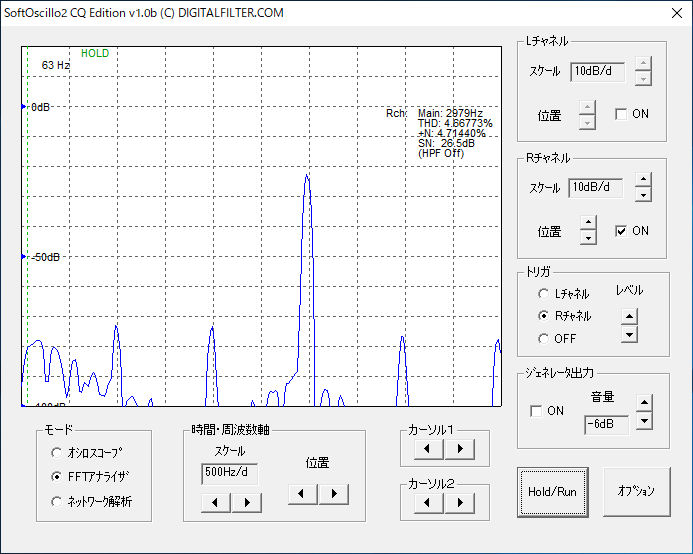
\includegraphics[width=\textwidth,height=50mm]{./documents/05/0109-dsPICマイコンプログラミング1/images/3k-fft.png}
\caption{subject}\label{fig:3k-fft}
}
\end{figure}

\begin{figure}
\hypertarget{fig:3k-fft}{%
\centering
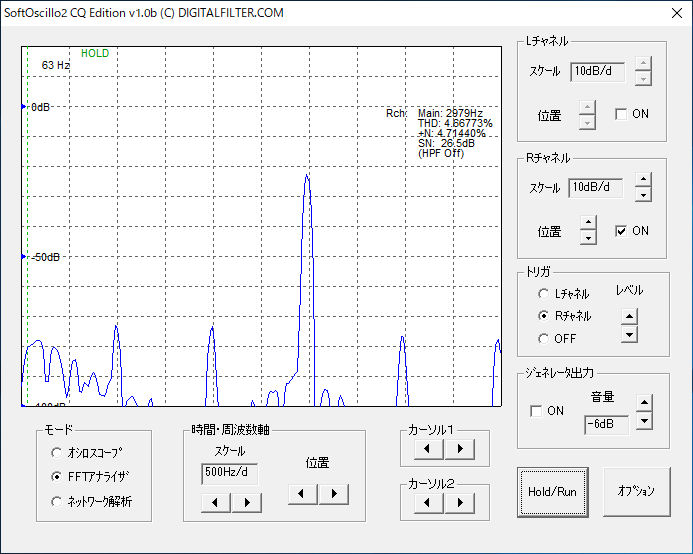
\includegraphics[width=\textwidth,height=50mm]{./documents/05/0109-dsPICマイコンプログラミング1/images/3k-fft.png}
\caption{subject}\label{fig:3k-fft}
}
\end{figure}

\clearpage

\hypertarget{ux8ab2ux984c-4}{%
\subsection{課題 4}\label{ux8ab2ux984c-4}}

\begin{codelisting}

\caption{課題 4}

\hypertarget{lst:awesome-code}{%
\label{lst:awesome-code}}%
\begin{Shaded}
\begin{Highlighting}[numbers=left,,]
\PreprocessorTok{#include }\ImportTok{<p30F3013.h>}

\DataTypeTok{void}\NormalTok{ init_adc() \{}
\NormalTok{  TRISBbits.TRISB3 = }\DecValTok{1}\NormalTok{;  }\CommentTok{// RB1 as input}
\NormalTok{  ADPCFG = }\BaseNTok{0xFFF7}\NormalTok{;}
\NormalTok{  ADCHS = }\BaseNTok{0x0003}\NormalTok{;}
\NormalTok{  ADCON1 = }\BaseNTok{0x0044}\NormalTok{;}
\NormalTok{  ADCSSL = }\DecValTok{0}\NormalTok{;}
\NormalTok{  ADCON2 = }\BaseNTok{0x0000}\NormalTok{;}
\NormalTok{  ADCON3 = }\BaseNTok{0x0113}\NormalTok{;}
\NormalTok{  ADCON1bits.ADON = }\DecValTok{1}\NormalTok{;  }\CommentTok{// ADC on}
\NormalTok{\}}

\DataTypeTok{void}\NormalTok{ init_timer() \{}
\NormalTok{  INTCON1bits.NSTDIS = }\DecValTok{0}\NormalTok{;}
\NormalTok{  INTCON2bits.ALTIVT = }\DecValTok{1}\NormalTok{;  }\CommentTok{// 代替ベクタを使用}
\NormalTok{  TMR3 = }\BaseNTok{0x0000}\NormalTok{;           }\CommentTok{// clear counter register}
\NormalTok{  PR3 = }\DecValTok{1024}\NormalTok{ - }\DecValTok{1}\NormalTok{;          }\CommentTok{// set period register}
\NormalTok{  IFS0 = }\BaseNTok{0x0000}\NormalTok{;           }\CommentTok{// clear all interrupt}
\NormalTok{  T3CON = }\BaseNTok{0x8000}\NormalTok{;          }\CommentTok{// start TIMER3 on}
\NormalTok{  IPC1 = }\BaseNTok{0x5000}\NormalTok{;}
\NormalTok{  IPC2 = }\BaseNTok{0x3000}\NormalTok{;}
\NormalTok{  IEC0 = }\BaseNTok{0x0880}\NormalTok{;}

\NormalTok{  TRISBbits.TRISB9 = }\DecValTok{0}\NormalTok{;  }\CommentTok{// OC2 pin as output}
\NormalTok{  OC2CON = }\BaseNTok{0x0006}\NormalTok{;       }\CommentTok{// PWM mode}
\NormalTok{  TMR2 = }\BaseNTok{0x0000}\NormalTok{;         }\CommentTok{// clear counter register}
\NormalTok{  PR2 = }\DecValTok{1024}\NormalTok{ - }\DecValTok{1}\NormalTok{;        }\CommentTok{// set period register}
\NormalTok{  T2CON = }\BaseNTok{0x8000}\NormalTok{;        }\CommentTok{// start TIMER2 on}
\NormalTok{  OC2RS = }\DecValTok{0}\NormalTok{;}
\NormalTok{\}}

\DataTypeTok{int}\NormalTok{ Resultdata, Msec = }\DecValTok{0}\NormalTok{, flag = }\DecValTok{0}\NormalTok{;}

\DataTypeTok{void}\NormalTok{ _ISR _AltT3Interrupt(}\DataTypeTok{void}\NormalTok{) \{}
  \ControlFlowTok{while}\NormalTok{ (!IFS0bits.ADIF);}
\NormalTok{  Resultdata = ADCBUF0;}
\NormalTok{  OC2RS = Resultdata >> }\DecValTok{2}\NormalTok{;}
\NormalTok{  IFS0bits.ADIF = }\DecValTok{0}\NormalTok{;}
\NormalTok{  IFS0bits.T3IF = }\DecValTok{0}\NormalTok{;  }\CommentTok{// タイマ3割り込みフラグクリア}
\NormalTok{\}}

\DataTypeTok{int}\NormalTok{ main(}\DataTypeTok{void}\NormalTok{) \{}
\NormalTok{  init_adc();}
\NormalTok{  init_timer();}
  \ControlFlowTok{while}\NormalTok{ (}\DecValTok{1}\NormalTok{);}
\NormalTok{\}}
\end{Highlighting}
\end{Shaded}

\end{codelisting}

\clearpage

\hypertarget{ux307eux3068ux3081}{%
\section{まとめ}\label{ux307eux3068ux3081}}

室内の温度と同程度の温度がシリアルモニタに出力されたとともに,
センサモジュールを指などで触れることできちんと温湿度の上昇を確認できたことより実験は成功したと考える.

\hypertarget{ux53c2ux8003ux6587ux732e}{%
\section{参考文献}\label{ux53c2ux8003ux6587ux732e}}

\begin{itemize}
\tightlist
\item
  AE-BME280 取扱説明書 \textbar{} 秋月電子通商

  \begin{itemize}
  \tightlist
  \item
    https://akizukidenshi.com/download/ds/akizuki/AE-BME280\_manu\_v1.1.pdf
  \end{itemize}
\end{itemize}

\end{document}
